The main goal in this project is to detect and identify balls. There are different approaches to solving this problem, where some ideas concentrate on solving both problems at once by identifying balls directly and thereby also implicitly detecting them. Other solutions, like the one used in this project, does the detecting first to determine the regions of interest and then extract further data from the regions for use in the identification process.

The advantage of the former is that the computation can be done in one pass and thereby potentially reduce computation time. Features that are used to identify the balls can in this way also be used in the detection process which might create a more robust detection because that a identified ball implies a good detection.

The advantage of the latter is that further information is available when all balls are detected, opposite to a situation where a ball is being identified without the knowledge of any other detected balls on the table.

\subsection{Solution ideas}

\subsubsection{Template matching}
By constructing templates that represents the different ways a ball can be turned, e.g. with number up, stripe turned different ways, template matching can be applied to identify balls on the table. This method will do detection and matching at the same time and thereby utilize the information contained in the template, concerning color and shape, to both find an accurate matching position and at the same time identify the ball which will be equal to the template in use.

Using this method requires that a sufficient number of templates are created to cover the possible ways that a ball is turned. Templates are created by either sampling balls in many different positions, or generating them using the knowledge of color and looks of a ball. Problems arise when similar colored balls are in close proximity, as this will create matches in positions between the balls.

The template punishes colors inside the ball that are not in the same position as they are in the template, e.g. the number and the stripe in striped balls. 

The method is also has high complexity for the reason that each template has to be matched against the entire table.

Experiments with matching a simple one-colored template against the balls proved inaccurate, and the template also introduced matches on the edges of balls if the color intensity was high there.

\subsubsection{Histogram backprojection}
Using histograms extracted from balls in training data, the histograms are backprojected against the entire image of the pool table. This is done by computing the histogram inside a mask in every image position, and then assigning a score to the position by measuring the difference between the sampled and model training histogram.

This process is similar to the template matching described above, but instead of taking into account the structure of the image, i.e. where the different colors are inside the ball, this method evaluates the distribution of the colors regardless of structure.
\begin{figure}[H]
  \centering
  \subfloat[Good match]{\label{fig:backProjectGood}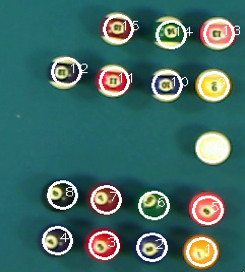
\includegraphics[width=0.48\textwidth]{images/backprojectGood.png}}
  \quad           
  \subfloat[Bad match]{\label{fig:backProjectBad}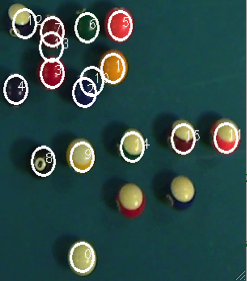
\includegraphics[width=0.48\textwidth]{images/backprojectBad.png}}
   \caption{Results of the backprojection method. Labeled white circles indicate identified balls.}
  \label{fig:backprojectResults}
\end{figure}
Backprojection has some problems because of the different ways that a ball can face. The measure of similarity between the histograms is dependent of the distributions to have the same kind of structure. If the two histograms are equal, but one is shifted, the output will be that they are different. A simpler comparisson where e.g. only the mean is used to measure how close the ball distribution is to the model.

Figure \ref{fig:backprojectResults} shows results of experiments of backprojection methods. The model histograms that results in a good match against \ref{fig:backProjectGood}, has problems in \ref{fig:backProjectBad} where the balls are facing differently.

\subsubsection{BLOB analysis}
The uniform color of the table cloth can be utilized to apply a threshold to the image resulting in BLOBs representing ball locations. The BLOBs can be separated using morphology operations to separate balls in close proximity. The center position of BLOBs or a feature like the bounding circle, can be used to mark the center point of a ball. Pixels that are inside a BLOB is extracted for further processing to identify the ball.

As will be mentioned later in this section, the idea of using this kind of segmentation to reduce the ROI is not a bad idea, but using the pixels in a BLOB can cause problems if all ball pixels are not included, or pixels that does not belong to the BLOB are included. This happens frequently when balls are laying too close to produce separate BLOBs, but instead ends up as one large BLOB containing pixels from several balls.

\subsubsection{Chosen Solution: Ball probability estimation}
The solution used in this project uses the two-step process by first detecting ball positions and thereafter identifying the detected balls.

In this solution, a pool ball consists of one only one primary color and white. By counting the number of pixels inside a circular area which satisfies this, a ball probability can be estimated. The positions in the image having the highest probabilities are considered ball locations and can be passed on to the identifier.

The identification process can be separated into two steps: determining if the ball is striped and determining the color of the ball. The ball is considered striped if the ratio between white and colored pixels are above a certain level. The color is determined by comparing the distribution of the color in the detected position with known training data.